\documentclass[12pt]{report}
\usepackage{graphicx}
\usepackage{subfig}
\usepackage{listings}
\usepackage{hyperref}

\begin{document}
\lstset{language=Python}

\title{Homework 1 - Applied Machine Learning}
\author{Tim Delisle and Sam Raudabaugh}
\date{09/15/2015}
\maketitle


\noindent{{\large 2. Titanic Disaster}}

For this assignment, we competed in the Titanic dataset challenge on Kaggle. Our goal was to train a logistic regression classifier that uses passenger data, such as age and gender, to predict who
survived.

It turns out that the \verb+scikit-learn+ package contains a \verb+LogisticRegression+ model that we can use for this very purpose. Before we can train such a model, however, we need to clean the
data provided by Kaggle, fill in missing values, and select a combination of features for the model to examine.

Preparation of the training and test data occurs within \verb+munge_data()+ in the attached code. For the logistic regression training and predicting to work, input data must be numeric, so much
of our preparation involves mapping categorical data (i.e. \verb+Sex+ and \verb+Port of Embarkation+) to numeric values (\verb+Sex_enum+ and \verb+Embarked_enum+).

Next, we fill in missing data - in particular, \verb+Age+ and \verb+Fare+ - with a dummy value derived from the rest of the dataset. To determine the best dummy values, it is helpful to examine
the attached histograms in Figure 1. We see that the distributions of ages and fares are both highly skewed, so a median value might be more appropriate than a mean. One sophisticated approach,
borrowed from \href{https://www.kaggle.com/c/titanic/details/getting-started-with-python-ii}{Kaggle's "Getting Started With Python II" guide}, is to use the median fare/age for a given gender
and passenger's socioeconomic status, which will hopefully better represent typical passengers.

\begin{figure}
\centering
\subfloat[training data]{
  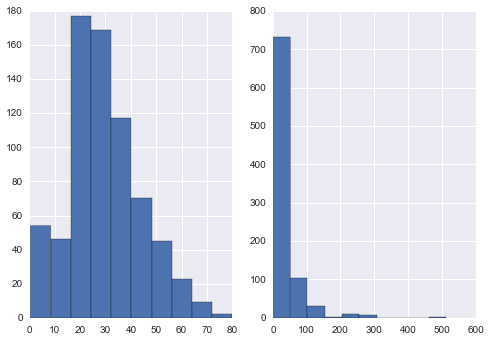
\includegraphics[width=50mm]{figures/train-age-fare.png}
}
\subfloat[test data]{
  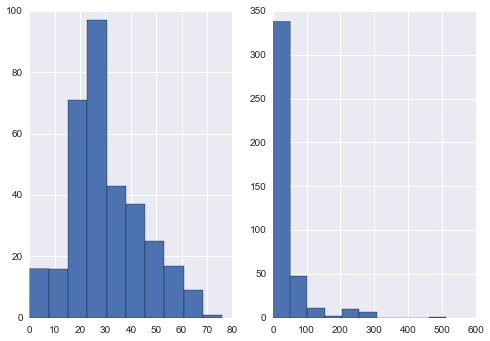
\includegraphics[width=50mm]{figures/test-age-fare.png}
}
\caption{Age (left) and fare (right) distributions}
\end{figure}

A couple of features in the dataset were ignored, namely \verb+Ticket+ and \verb+Cabin+. The difficulty of mapping these categorical values, which seem irrelevant, would likely outweigh any
benefits. Additionally, the values for \verb+Cabin+ were largely missing.

Following \href{https://www.kaggle.com/c/titanic/details/getting-started-with-python-ii}{the Kaggle article}, we constructed two new features from the dataset:
\verb+FamilySize+, obtained simply by adding together the number of siblings, spouses, parents and children aboard, and \verb+Age*Class+, obtained by multiplying age by the passenger's
socioeconomic status (1 for upper class, 2 for middle class, 3 for lower class), since both older and lower class passengers had a lower likelihood of survival.

At each decision step, we test the usefulness of a combination of features with a 10 fold cross-validation technique, which uses the code from Michael Wilber's lecture working with the \verb+cross_validation+
module in \verb+scikit-learn+ as a starting point.
Using \verb+FamilySize+ and \verb+Age*Class+ in place of \verb+Age+ both produced higher cross-validation scores.

We also experimented with pulling out the titles of each passenger's name and categorizing them in different ways. The first strategy was a binary approach with only pedestrian and non-pedestrian titles,
while the second strategy used 5 title types: pedestrian, honorary, academic, military, or religious. The latter approach resulted in higher cross-validation scores, though neither approach seemed to affect the Kaggle test results.
For reference, the attached code makes use of the second strategy, defined in \verb+get_title_type()+.

After running our solution on the test dataset, we submitted the results to Kaggle and received a score of 0.75598 as shown in Figure 2. For future improvements, experimenting with another model,
such as a random forest classifier, is recommended.
\begin{figure}
\centering
  
\includegraphics[width=150mm]{figures/kaggle-titanic.png}
\caption{Kaggle result for Titanic challenge}
\end{figure}
\newpage
\noindent{{\large Written 1. Variance of a sum}}
\\\\
Show var[X+Y] = var[X] + var[Y] + 2cov[X,Y].
\\\\
$var[X+Y] = cov[X+Y, X+Y]$
\\\\
By definition of covariance:
\\
$var[X+Y] = E[(X+Y)(X+Y)] - E[X+Y]E[X+Y]$
\\\\
$var[X+Y] = E[(X^2+2XY+Y^2]-(E[X]+E[Y])(E[X]+E[Y])$
\\\\
$var[X+Y] = E[X^2]-E[X]E[X] + E[Y^2]-E[Y]E[Y] + E[XY]-E[X]E[Y] + E[XY]-E[X]E[Y]$
\\\\
$var[X+Y] = cov[X,X] + cov[Y,Y] + cov[X,Y] + cov[X,Y]$
\\\\
$var[X+Y] = var[X] + var[Y] + 2cov[X,Y]$
\\\\
\noindent{{\large Written 2. Bayes rule for medical diagnosis}}
\\\\
Let $D$ refer to the event that you have the disease, and $TP$ refer to the event that you tested positive. Then:
\\\\
$P(D|TP) = \frac{P(D)P(TP|D)}{P(TP)}$
\\\\
Given $P(D) = 0.0001$ and $P(TP|D) = 0.99$, we only need to derive $P(TP)$.
\\\\
$P(TP) = P(TP|D)P(D)+P(TP|D')P(D')$
\\\\
Finally, with $P(TP|D') = 0.01$ and $P(D') = 0.9999$:
\\\\
$P(D|TP) = \frac{P(D)P(TP|D)}{P(TP|D)P(D)+P(TP|D')P(D')} = \frac{0.0001*0.99}{0.99*0.0001+0.01*0.9999} = 0.0098$
\newpage
\noindent{{\large Written 3a. Derivative of sigmoid function}}
\\\\
Given $\sigma(a) = \frac{1}{1+e^{-a}} = (1+e^{-a})^{-1}$
\\\\
$\frac{d\sigma(a)}{da} = -(1+e^{-a})^{-2}*-e^{-a}$
\\\\
$\frac{d\sigma(a)}{da} = \frac{e^{-a}}{(1+e^{-a})^2}$
\\\\
$\frac{d\sigma(a)}{da} = \frac{1}{1+e^{-a}}\left(\frac{e^{-a}}{1+e^{-a}}\right)$
\\\\
$\frac{d\sigma(a)}{da} = \frac{1}{1+e^{-a}}\left(\frac{1+e^{-a}}{1+e^{-a}} - \frac{1}{1+e^{-a}}\right)$
\\\\
$\frac{d\sigma(a)}{da} = \sigma(a)\left(1-\sigma(a)\right)$
\newpage
\noindent{{\large Written 3b. Gradient of log likelihood}}
\\\\
Given $l(\beta)=\sum_{i=1}^N\{y_ilogp(x_i;\beta)+(1-y_i)log(1-p(x_i;\beta))\}$
\\\\
$\frac{\delta l(\beta)}{\delta\beta}=\sum_{i=1}^N\frac{\delta}{\delta\beta}y_ilogp(x_i;\beta)+\sum_{i=1}^N\frac{\delta}{\delta\beta}(1-y_i)log(1-p(x_i;\beta))$
\\\\
Derive individual $\frac{\delta}{\delta\beta}$ terms:
\\\\
$\frac{\delta}{\delta\beta}y_ilogp(x_i;\beta)=y_i\cdot\frac{1}{p(x_i;\beta)}\cdot\frac{\delta}{\delta\beta}p(x_i;\beta)$
\\\\
$\frac{\delta}{\delta\beta}y_ilogp(x_i;\beta)=x_iy_i\cdot\frac{1}{p(x_i;\beta)}\cdot p(x_i;\beta)(1-p(x_i;\beta))=x_iy_i(1-p(x_i;\beta))$
\\\\
and:
\\\\
$\frac{\delta}{\delta\beta}(1-y_i)log(1-p(x_i;\beta))=(1-y_i)\frac{1}{1-p(x_i;\beta)}\cdot\frac{\delta}{\delta\beta}(1-p(x_i;\beta))$
\\\\
$\frac{\delta}{\delta\beta}(1-y_i)log(1-p(x_i;\beta))=\frac{1-y_i}{1-p(x_i;\beta)}\cdot-x_ip(x_i;\beta)(1-p(x_i;\beta))$
\\\\
$\frac{\delta}{\delta\beta}(1-y_i)log(1-p(x_i;\beta))=-x_i(1-y_i)p(x_i;\beta)$
\\\\
Plugging the terms into the original gradient, we simplify to the desired form:
\\\\
$\frac{\delta l(\beta)}{\delta\beta}=\sum_{i=1}^Nx_iy_i(1-p(x_i;\beta))-x_i(1-y_i)p(x_i;\beta)$
\\\\
$\frac{\delta l(\beta)}{\delta\beta}=\sum_{i=1}^Nx_i(y_i-y_ip(x_i;\beta)-(1-y_i)p(x_i;\beta))=\sum_{i=1}^Nx_i(y_i-p(x_i;\beta))$
\newpage
\noindent{{\large Written 3c. Proof that log likelihood Hessian is positive definite}}
\\\\
In order to prove that $X^TWX$ is positive definite, we must show that the scalar $v^TX^TWXv > 0$ for every $v$, which is any non-zero column vector of real numbers.
\\\\
Because $W$ is a diagonal matrix of non-negative real values $w_i$, we can absorb $W$ into $X$ and refactor $X^TWX$ into the following form:
\\\\
$X^TWX = Q^TQ$
\\\\
where each element of $Q$ is equal to the element at the same $i^{th}$ row and $j^{th}$ column in $X$, multiplied by $\sqrt{w_i}$.
\\\\
Plugging this new form into the expression $v^TX^TWXv$, we find that the expression can be represented as the inner product of $Qv$:
\\\\
$v^TX^TWXv = v^TQ^TQv = (Qv)^TQv = ||Qv||$
\\\\
which is a scalar representing the magnitude of a vector in Euclidian space, therefore it cannot be negative. Assuming nondegeneracy in the data (no duplicate inputs $x_i$), it also cannot be 0.
Therefore:
\\\\
$||Qv|| = v^TX^TWXv > 0$
\end{document}
